\chapter{Growth Yield Analysis}
\label{chap:yield_analysis}






\section{article2}
\begin{figure}
    \centering
    \includegraphics[width=\textwidth]{4_Properties/From_Article2/Figure2.png}
    \caption{Top-view SEM images of arrays with grown III-V nanowires. The \qty{70}{\nm}, \qty{140}{\nm}, \qty{210}{\nm}, and \qty{280}{\nm} wide wires are shown from top to bottom. The arrays on the left contain structures grown from a seed surface parallel to the template direction, while those on the right are grown from seed surfaces that are tilted concerning the template. On the bottom left of the images, the three main elements of the arrays are highlighted in green (silicon seed), red (III-V nanowires), and blue (template opening).}
    \label{fig:arrays}
\end{figure}

Figure~\ref{fig:arrays} shows growth results from sample 1 of arrays containing template nanotubes of four different widths (\qty{70}{nm}, \qty{140}{nm}, \qty{210}{nm}, and \qty{280}{nm}). Each array contains 66 nanowires (in red) grown from silicon (in green) and arranged in 33 pairs. Each pair of wires shares the same template opening (in blue). 
\par
Each wire in the array can be identified by its row, opening, and position relative to the latter. Each row is numbered from 1 to 11, starting at the bottom of the array. The template openings are marked by letters A, B, or C; the wires connected to the opening to the left (l) or right (r) can be easily distinguished. Therefore, a string such as 9Br identifies a single wire in the array. 
\par
Our growth methodology aims to select and maintain a single \hkl{111}\(_B\) facet as the nanowire's growth front. If a III-V wire end-surface is multi-faceted or not parallel to the \acs{si} seed facet, the wire is classified as defective in this study without requiring a further in-depth STEM analysis. This first distinction allows the evaluation of the fraction of "perfect" wires, defining a growth yield. 
\par
In Figure~\ref{fig:arrays}, the \qty{280}{nm} tilted arrays present some defective wires in 11Al, 6Cr, and 7Cr; however, the other wires in each pair (11Ar, 6Cl, and 7Cl) appear “perfect”. As is evident in the case of wire 6Cr, the wire grew into an unpredictable shape after nucleation. It is unclear if the source of defective wires can be attributed solely to the nucleation step, as there are other sites (\qty{70}{nm} tilted 6Cl, \qty{140}{nm} perpendicular 2Br, 11Br, and \qty{280}{nm} perpendicular 7Br) that present a defective wire and fully covered seed. However, this finding suggests that nucleation does play an important role in the following growth facet selection.


\begin{figure}
    \centering
    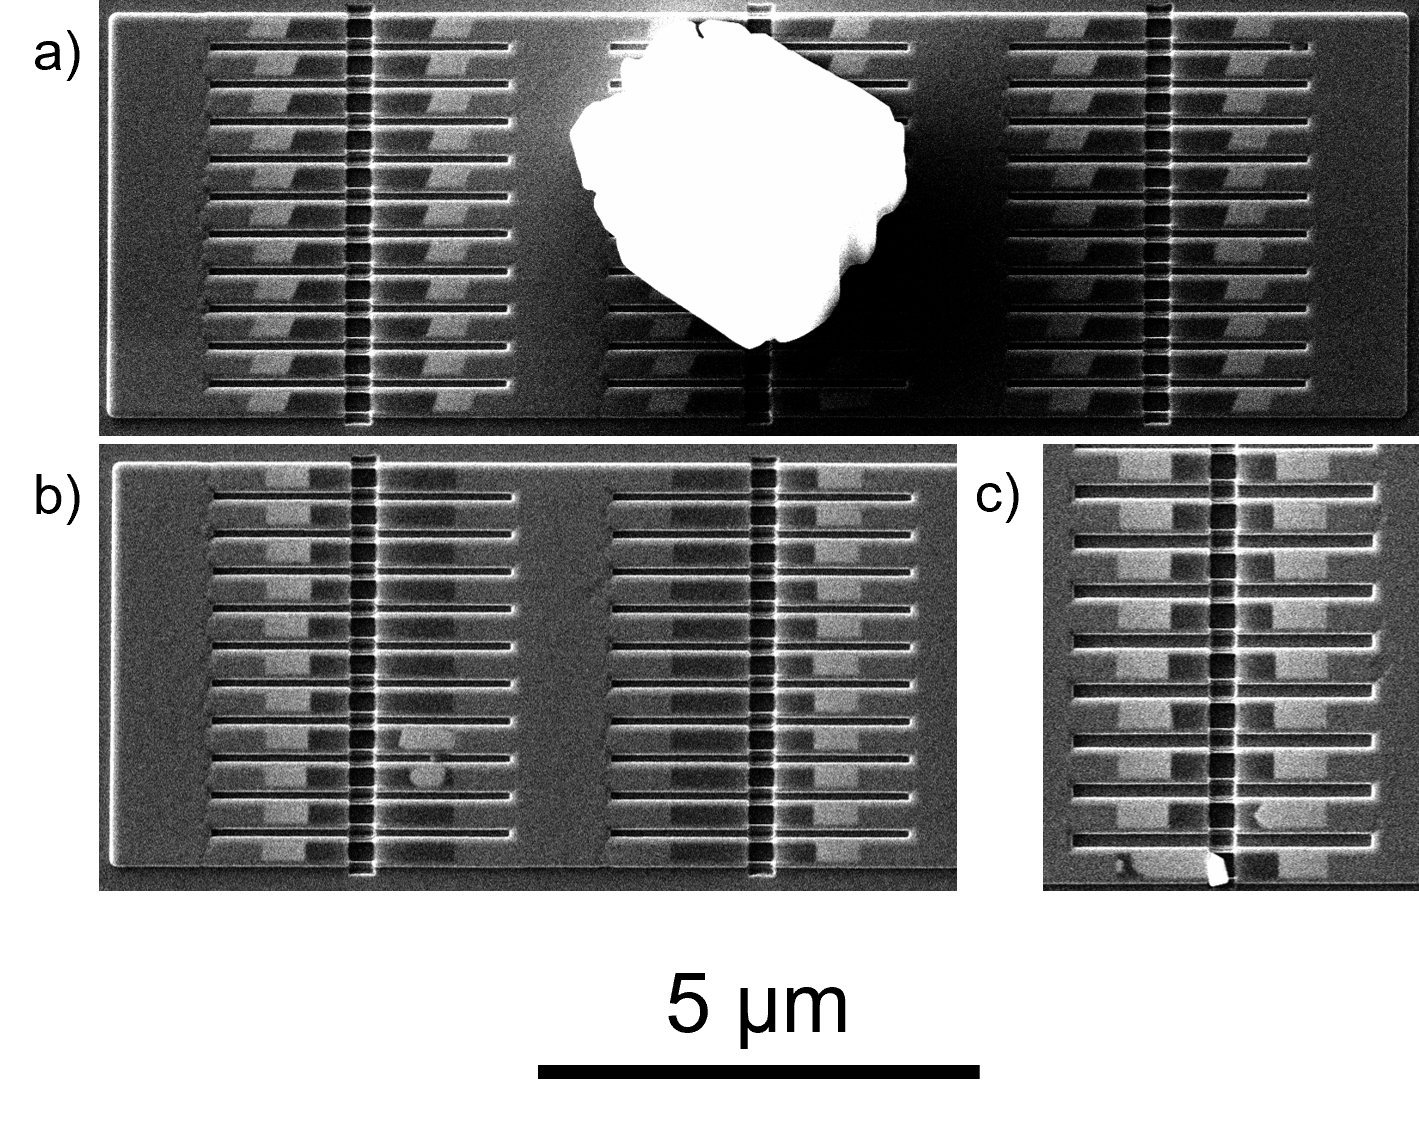
\includegraphics[width=\columnwidth]{4_Properties/From_Article2/Figure3.png}
    \caption{Examples of failure situations for TASE grown wires. (a) large parasitic crystal obstructing many growth sites. (b) multiple seeds do not show nucleation of III-V material at all, while one site shows parasitic nucleation inside the template. (c) in the bottom row, after initial nucleation on the \acs{si}, a parasitic crystal developed inside the template and grew out of it.}
    \label{fig:failures}
\end{figure}

Another parameter that negatively affects the growth yield is the loss of growth selectivity and the resulting parasitic growth. This is ascribed to impurities or surface features promoting nucleation. An example of this is shown in Figure~\ref{fig:failures}.a, where a single defect of this kind affects many wires. Figure~\ref{fig:failures}.b also shows sites where parasitic nucleation occurred within templates and, seed-sites that did not undergo III-V on \acs{si} nucleation, likely because of the lingering of a passivating \acs{sio2} layer on the \acs{si} seed surface. This happened despite the proximity to other correctly-grown wires. Finally, 
Figure~\ref{fig:failures}.c bottom row illustrates an example where, after the initial nucleation event, the channel was obstructed by a parasitic nucleation growth within the channel, which extends outside the template. This type of growth configuration can potentially cause deposits similar to that in Figure~\ref{fig:failures}.a.

\subsection{Yield study}

\sisetup{detect-all = true}
\begin{table}
    \centering
    \begin{tabular}{l|ccccccc}
        \hline
         & \multicolumn{7}{c}{Defect categories and occurrence} \\ 
         & $\begin{matrix} \text{Wrong} \\ \text{Facet} \end{matrix}$ & $\begin{matrix} \text{Hidden by} \\ \text{Parasitic} \end{matrix}$ & $\begin{matrix} \text{Oxide} \\ \text{Nucleated} \end{matrix}$ & $\begin{matrix} \text{Seed} \\ \text{Exposed} \end{matrix}$ & Long & Short & Ungrown \\ 
        \hline \hline
         & & & & & & & \\
        Sample 1 & \num{164} & \num{230} & \num{2} & \num{0} & \num{5} & \num{204} & \num{61} \\ 
        \hline
        Parallel & \num{81} & \num{170} & \num{1} & \num{0} & \num{4} & \num{0} & \num{0} \\
        \textit{\% of category} & \textit{\qty{49.4}{\%}} & \textit{\qty{77.9}{\%}} & \textit{\qty{50}{\%}} & \textit{-} & \textit{\qty{80}{\%}} & \textit{\qty{0}{\%}} & \textit{\qty{0}{\%}} \\ 
        \hline
        Tilted & \num{83} & \num{51} & \num{1} & \num{0} & \num{1} & \num{204} & \num{61} \\
        \textit{\% of category} & \textit{\qty{50.6}{\%}} & \textit{\qty{22.1}{\%}} & \textit{\qty{50}{\%}} & \textit{-} & \textit{\qty{20}{\%}} & \textit{\qty{100}{\%}} & \textit{\qty{100}{\%}} \\ 
        \hline
         & & & & & & & \\
        Sample 2 & \num{204} & \num{257} & \num{15} & \num{8} & \num{3} & \num{7} & \num{20} \\ 
        \hline
        Parallel & \num{127} & \num{145} & \num{6} & \num{4} & \num{1} & \num{5} & \num{20} \\
        \textit{\% of category} & \textit{\qty{62.3}{\%}} & \textit{\qty{56.4}{\%}} & \textit{\qty{40}{\%}} & \textit{\qty{50}{\%}} & \textit{\qty{33.3}{\%}} & \textit{\qty{71.4}{\%}} & \textit{\qty{100}{\%}} \\ 
        \hline
        Tilted & \num{77} & \num{112} & \num{9} & \num{4} & \num{2} & \num{2} & \num{0} \\
        \textit{\% of category} & \textit{\qty{37.7}{\%}} & \textit{\qty{43.6}{\%}} & \textit{\qty{60}{\%}} & \textit{\qty{50}{\%}} & \textit{\qty{66.7}{\%}} & \textit{\qty{28.6}{\%}} & \textit{\qty{0}{\%}} \\ 
        \hline
        & & & & & & & \\
        \textbf{Total} & \textbf{\num{368}} & \textbf{\num{487}} & \textbf{\num{17}} & \textbf{\num{8}} & \textbf{\num{8}} & \textbf{\num{211}} & \textbf{\num{81}} \\
        \hline
    \end{tabular}
    \caption{Distribution of failure types for samples 1 and 2. Each sample's total is broken down between wires grown parallel to or tilted away from the \hkl<111> direction. Percentages for these two sub-categories and an overall total are given.}
    \label{tab:failures}
\end{table}
\sisetup{detect-none = true}

A survey of the arrays was carried out using samples 1 and 2, and involved \num{15840} individual nanowires grown in \num{240} arrays grouped in \num{5} locations per sample. The areas investigated were the top left of the chips as well as randomly selected locations throughout it. Wires need to have two parallel visible \hkl{111} seed and end facets of equal length, and they need to have nucleated directly on the \acs{si} seed covering it in its entirety for them to be considered "perfect". Of the \num{15840} total wires \num{14660} match these criteria, totalling a global yield of \qty{92.55}{\%}.
\par
Of the \num{7920} wires imaged for each sample, \num{7254} grew successfully in sample 1, and \num{7406} grew successfully in sample 2, resulting in a corresponding growth yield of \qty{91.59}{\%} and \qty{93.51}{\%}. This result indicates that the different heterointerfaces of samples 1 and 2 do not significantly impact the growth yield. 
\par
Further analysis was carried out within each sample by comparing the template growth yield parallel to the \hkl<111> direction, and those tilted away from it. A larger number (\num{9504} out of \num{15840}) of wires of the first configuration were measured. For sample 2, the parallel and tilted configurations resulted in comparable growth yields of \qty{93.73}{\%} and \qty{93.75}{\%}, while sample 1 showed \qty{94.84}{\%} and \qty{86.71}{\%} growth yields for the same configurations. The larger difference in growth yields for parallel and tilted templates in sample 1 can be explained by one of the fivcategorisedselected locations containing tilted arrays, falling in an area of the chip with many nucleation issues. This area is reflected in Table~\ref{tab:failures} where sample 1 has more short and ungrown wires.
\par
The total of \num{1180} nanowires that experienced growth failure are categorised based on the type of failure they experienced. Table~\ref{tab:failures} breaks down the number of defective wires for each sample between parallel and tilted templates, on a per-category basis. The first category, labelled "wrong facet", groups wires which terminate with either a multi-faceted surface or in a single facet that is not parallel to the seed surface, and accounts for \num{368} wires (\qty{31.2}{\%} of the total defective wires). The second and largest category comprises wire locations hidden by a parasitic crystal (\num{461} wires or \qty{39.0}{\%} of the total failures). From a total of \num{240} arrays, \num{32} are affected by one or more parasitic crystals. Still, the parasitic crystals hide close to \num{15} (\num{14.87} on average) locations for nanowire growth in each of these arrays. The "oxide nucleated" category contains all the cases where a III-V crystal nucleated randomly inside a template instead on the \acs{si} seed and counts \num{17} wires, \qty{1.4}{\%} of the total. The wires in the category "seed exposed" have the expected end facet, but did not fully cover the entire seed surface, leaving some of it exposed (\num{8} wires, \qty{0.7}{\%}). The category "long" comprises wires that were significantly longer than the others but did not have other defects, accounting for \qty{0.7}{\%} of the defective wires for a total of \num{8}. The last two categories are abnormally short wires and ungrown wires, with \num{211} (\qty{20.1}{\%}) and \num{81} (\qty{6.9}{\%}) counts each. These two categories of wires are more common in the area which presented nucleation iCharacterisation1.